%% uncomment to list all files in log
%\listfiles

\documentclass[12pt]{report}


\usepackage{fontspec}

%\setmainfont[Scale=MatchLowercase]{Lucida Bright}
%\setmonofont{FreeMono}
%\setmonofont{Source Code Pro}
\setmonofont[Scale=MatchLowercase]{Ubuntu Mono}

\usepackage[headings]{fullpage}

% national use characters 
%\usepackage{inputenc}

% ams mathematical symbols
\usepackage{amsmath,amssymb}

% added to support pandoc highlighting
\usepackage{microtype}

\usepackage{makeidx}

% add index and bibliographies to table of contents
\usepackage[nottoc]{tocbibind}

% postscript courier and times in place of cm fonts
%\usepackage{courier}
%\usepackage{times}

% extended coloring
\usepackage{color}
\usepackage[table,dvipsnames]{xcolor}
\usepackage{colortbl}

% advanced date formating
\usepackage{datetime}

%support pandoc code highlighting
\usepackage{fancyvrb}
\DefineShortVerb[commandchars=\\\{\}]{\|}
\DefineVerbatimEnvironment{Highlighting}{Verbatim}{commandchars=\\\{\}}
% Add ',fontsize=\small' for more characters per line

%tango style colors
% \usepackage{framed}
% \definecolor{shadecolor}{RGB}{255,255,255}
% \newenvironment{Shaded}{\begin{snugshade}}{\end{snugshade}}
% \newcommand{\KeywordTok}[1]{\textcolor[rgb]{0.13,0.29,0.53}{\textbf{{#1}}}}
% \newcommand{\DataTypeTok}[1]{\textcolor[rgb]{0.13,0.29,0.53}{{#1}}}
% \newcommand{\DecValTok}[1]{\textcolor[rgb]{0.00,0.00,0.81}{{#1}}}
% \newcommand{\BaseNTok}[1]{\textcolor[rgb]{0.00,0.00,0.81}{{#1}}}
% \newcommand{\FloatTok}[1]{\textcolor[rgb]{0.00,0.00,0.81}{{#1}}}
% \newcommand{\CharTok}[1]{\textcolor[rgb]{0.31,0.60,0.02}{{#1}}}
% \newcommand{\StringTok}[1]{\textcolor[rgb]{0.31,0.60,0.02}{{#1}}}
% \newcommand{\CommentTok}[1]{\textcolor[rgb]{0.56,0.35,0.01}{\textit{{#1}}}}
% \newcommand{\OtherTok}[1]{\textcolor[rgb]{0.56,0.35,0.01}{{#1}}}
% \newcommand{\AlertTok}[1]{\textcolor[rgb]{0.94,0.16,0.16}{{#1}}}
% \newcommand{\FunctionTok}[1]{\textcolor[rgb]{0.00,0.00,0.00}{{#1}}}
% \newcommand{\RegionMarkerTok}[1]{{#1}}
% \newcommand{\ErrorTok}[1]{\textbf{{#1}}}
% \newcommand{\NormalTok}[1]{{#1}}

%espresso style colors
% \usepackage{framed}
% \definecolor{shadecolor}{RGB}{42,33,28}
% \newenvironment{Shaded}{\begin{snugshade}}{\end{snugshade}}
% \newcommand{\KeywordTok}[1]{\textcolor[rgb]{0.26,0.66,0.93}{\textbf{{#1}}}}
% \newcommand{\DataTypeTok}[1]{\textcolor[rgb]{0.74,0.68,0.62}{\underline{{#1}}}}
% \newcommand{\DecValTok}[1]{\textcolor[rgb]{0.27,0.67,0.26}{{#1}}}
% \newcommand{\BaseNTok}[1]{\textcolor[rgb]{0.27,0.67,0.26}{{#1}}}
% \newcommand{\FloatTok}[1]{\textcolor[rgb]{0.27,0.67,0.26}{{#1}}}
% \newcommand{\CharTok}[1]{\textcolor[rgb]{0.02,0.61,0.04}{{#1}}}
% \newcommand{\StringTok}[1]{\textcolor[rgb]{0.02,0.61,0.04}{{#1}}}
% \newcommand{\CommentTok}[1]{\textcolor[rgb]{0.00,0.40,1.00}{\textit{{#1}}}}
% \newcommand{\OtherTok}[1]{\textcolor[rgb]{0.74,0.68,0.62}{{#1}}}
% \newcommand{\AlertTok}[1]{\textcolor[rgb]{1.00,1.00,0.00}{{#1}}}
% \newcommand{\FunctionTok}[1]{\textcolor[rgb]{1.00,0.58,0.35}{\textbf{{#1}}}}
% \newcommand{\RegionMarkerTok}[1]{\textcolor[rgb]{0.74,0.68,0.62}{{#1}}}
% \newcommand{\ErrorTok}[1]{\textcolor[rgb]{0.74,0.68,0.62}{\textbf{{#1}}}}
% \newcommand{\NormalTok}[1]{\textcolor[rgb]{0.74,0.68,0.62}{{#1}}}

%kete style colors
% \newenvironment{Shaded}{}{}
% \newcommand{\KeywordTok}[1]{\textbf{{#1}}}
% \newcommand{\DataTypeTok}[1]{\textcolor[rgb]{0.50,0.00,0.00}{{#1}}}
% \newcommand{\DecValTok}[1]{\textcolor[rgb]{0.00,0.00,1.00}{{#1}}}
% \newcommand{\BaseNTok}[1]{\textcolor[rgb]{0.00,0.00,1.00}{{#1}}}
% \newcommand{\FloatTok}[1]{\textcolor[rgb]{0.50,0.00,0.50}{{#1}}}
% \newcommand{\CharTok}[1]{\textcolor[rgb]{1.00,0.00,1.00}{{#1}}}
% \newcommand{\StringTok}[1]{\textcolor[rgb]{0.87,0.00,0.00}{{#1}}}
% \newcommand{\CommentTok}[1]{\textcolor[rgb]{0.50,0.50,0.50}{\textit{{#1}}}}
% \newcommand{\OtherTok}[1]{{#1}}
% \newcommand{\AlertTok}[1]{\textcolor[rgb]{0.00,1.00,0.00}{\textbf{{#1}}}}
% \newcommand{\FunctionTok}[1]{\textcolor[rgb]{0.00,0.00,0.50}{{#1}}}
% \newcommand{\RegionMarkerTok}[1]{{#1}}
% \newcommand{\ErrorTok}[1]{\textcolor[rgb]{1.00,0.00,0.00}{\textbf{{#1}}}}
% \newcommand{\NormalTok}[1]{{#1}}
%end pandoc code hacks

% jodliterate colors
\usepackage{color}
\definecolor{shadecolor}{RGB}{248,248,248}
% j control structures 
\definecolor{keywcolor}{rgb}{0.13,0.29,0.53}
% j explicit arguments x y m n u v
\definecolor{datacolor}{rgb}{0.13,0.29,0.53}
% j numbers - all types see j.xml
\definecolor{decvcolor}{rgb}{0.00,0.00,0.81}
\definecolor{basencolor}{rgb}{0.00,0.00,0.81}
\definecolor{floatcolor}{rgb}{0.00,0.00,0.81}
% j local assignments
\definecolor{charcolor}{rgb}{0.31,0.60,0.02}
\definecolor{stringcolor}{rgb}{0.31,0.60,0.02}
\definecolor{commentcolor}{rgb}{0.56,0.35,0.01}
% primitive adverbs and conjunctions
%\definecolor{othercolor}{rgb}{0.56,0.35,0.01}   
\definecolor{othercolor}{RGB}{0,0,255}
% global assignments
\definecolor{alertcolor}{rgb}{0.94,0.16,0.16}
% primitive J verbs and noun names
\definecolor{funccolor}{rgb}{0.00,0.00,0.00}    

\usepackage{framed}
\newenvironment{Shaded}{}{}
\newcommand{\KeywordTok}[1]{\textcolor{keywcolor}{\textbf{{#1}}}}
\newcommand{\DataTypeTok}[1]{\textcolor{datacolor}{{#1}}}
%\newcommand{\DecValTok}[1]{\textcolor{decvcolor}{{#1}}}
\newcommand{\DecValTok}[1]{{#1}} 
\newcommand{\BaseNTok}[1]{\textcolor{basencolor}{{#1}}}
\newcommand{\FloatTok}[1]{\textcolor{floatcolor}{{#1}}}
\newcommand{\CharTok}[1]{\textcolor{charcolor}{\textbf{{#1}}}}
\newcommand{\StringTok}[1]{\textcolor{stringcolor}{{#1}}}
\newcommand{\CommentTok}[1]{\textcolor{commentcolor}{\textit{{#1}}}}
\newcommand{\OtherTok}[1]{\textcolor{othercolor}{{#1}}} 
\newcommand{\AlertTok}[1]{\textcolor{alertcolor}{\textbf{{#1}}}}
%\newcommand{\FunctionTok}[1]{\textcolor{funccolor}{{#1}}}
\newcommand{\FunctionTok}[1]{{#1}}
\newcommand{\RegionMarkerTok}[1]{{#1}}
\newcommand{\ErrorTok}[1]{\textbf{{#1}}}
\newcommand{\NormalTok}[1]{{#1}}

% headers and footers
\usepackage{fancyhdr}
\pagestyle{fancy}

\fancyhead{}
\fancyfoot{}

%\fancyhead[LE,RO]{\slshape \rightmark}
%\fancyhead[LO,RE]{\slshape \leftmark}
\fancyfoot[C]{\thepage}
%\headrulewidth 0.4pt
%\footrulewidth 0 pt

%\addtolength{\headheight}{\baselineskip}

%\lfoot{\emph{Analyze the Data not the Drivel}}
%\rfoot{\emph{\today}}

% subfigure handles figures that contain subfigures
%\usepackage{color,graphicx,subfigure,sidecap}
\usepackage{graphicx,sidecap}
\usepackage{subfigure}
\graphicspath{{./inclusions/}}

% floatflt provides for text wrapping around small figures and tables
\usepackage{floatflt}

% tweak caption formats 
\usepackage{caption} 
\usepackage{sidecap}
%\usepackage{subcaption} % not compatible with subfigure

\usepackage{rotating} % flip tables sideways

% complex footnotes
%\usepackage{bigfoot}

% weird logos \XeLaTeX
\usepackage{metalogo}

% source code listings
\usepackage{listings}

% long tables
% \usepackage{longtable}

\newcommand{\HRule}{\rule{\linewidth}{0.5mm}}

% map LaTeX cross references into PDF cross references
\usepackage[
            %dvips,
            colorlinks,
            linkcolor=blue,
            citecolor=blue,
            urlcolor=blue,   % magenta, cyan default        
            pdfauthor={John D. Baker},
            pdftitle={Analyze the Data not the Drivel},
            pdfsubject={Blog},
            pdfcreator={MikTeX+LaTeXe with hyperref package},
            pdfkeywords={blog,wordpress},
            ]{hyperref}
           
% custom colors
\definecolor{CodeBackGround}{cmyk}{0.0,0.0,0,0.05}    % light gray
\definecolor{CodeComment}{rgb}{0,0.50,0.00}           % dark green {0,0.45,0.08}
\definecolor{TableStripes}{gray}{0.9}                 % odd/even background in tables

\lstdefinelanguage{bat}
{morekeywords={echo,title,pushd,popd,setlocal,endlocal,off,if,not,exist,set,goto,pause},
sensitive=True,
morecomment=[l]{rem}
}

\lstdefinelanguage{jdoc}
{
morekeywords={},
otherkeywords={assert.,break.,continue.,for.,do.,if.,else.,elseif.,return.,select.,end.
,while.,whilst.,throw.,catch.,catchd.,catcht.,try.,case.,fcase.},
sensitive=True,
morecomment=[l]{NB.},
morestring=[b]',
morestring=[d]',
}

% latex size ordering - can never remember it
% \tiny
% \scriptsize
% \footnotesize
% \small
% \normalsize
% \large
% \Large
% \LARGE
% \huge
% \Huge
 
% listings package settings  
\lstset{%
  language=jdoc,                                % j document settings
  basicstyle=\ttfamily\footnotesize,            
  keywordstyle=\bfseries\color{keywcolor}\footnotesize,
  identifierstyle=\color{black},
  commentstyle=\slshape\color{CodeComment},     % colored slanted comments
  stringstyle=\color{red}\ttfamily,
  showstringspaces=false,                       
  %backgroundcolor=\color{CodeBackGround},       
  frame=single,                                
  framesep=1pt,                                 
  framerule=0.8pt,                             
  rulecolor=\color{CodeBackGround},   
  showspaces=false,
  %columns=fullflexible,
  %numbers=left,
  %numberstyle=\footnotesize,
  %numbersep=9pt,
  tabsize=2,
  showtabs=false,
  captionpos=b
  breaklines=true,                              
  breakindent=5pt                              
}

\lstdefinelanguage{JavaScript}{
  keywords={typeof, new, true, false, catch, function, return, null, catch, switch, var, if, in, while, do, else, case, break},
  ndkeywords={class, export, boolean, throw, implements, import, this},
  ndkeywordstyle=\color{darkgray}\bfseries,
  sensitive=false,
  comment=[l]{//},
  morecomment=[s]{/*}{*/},
  morestring=[b]',
  morestring=[b]"
}

% C# settings
\lstdefinestyle{sharpc}{
language=[Sharp]C,
basicstyle=\ttfamily\scriptsize, 
keywordstyle=\bfseries\color{keywcolor}\scriptsize,
framerule=0pt
}

% for source code listing longer than two use smaller font
\lstdefinestyle{smallersource}{
basicstyle=\ttfamily\scriptsize, 
keywordstyle=\bfseries\color{keywcolor}\scriptsize,
framerule=0pt
}

\lstdefinestyle{resetdefaults}{
language=jdoc,
basicstyle=\ttfamily\footnotesize,  
keywordstyle=\bfseries\color{keywcolor}\footnotesize,                                                               
framerule=0.8pt 
}

% APL UTF8 code points listed for lstlisting processing
\makeatletter
\lst@InputCatcodes
\def\lst@DefEC{%
 \lst@CCECUse \lst@ProcessLetter
  ^^80^^81^^82^^83^^84^^85^^86^^87^^88^^89^^8a^^8b^^8c^^8d^^8e^^8f%
  ^^90^^91^^92^^93^^94^^95^^96^^97^^98^^99^^9a^^9b^^9c^^9d^^9e^^9f%
  ^^a0^^a1^^a2^^a3^^a4^^a5^^a6^^a7^^a8^^a9^^aa^^ab^^ac^^ad^^ae^^af%
  ^^b0^^b1^^b2^^b3^^b4^^b5^^b6^^b7^^b8^^b9^^ba^^bb^^bc^^bd^^be^^bf%
  ^^c0^^c1^^c2^^c3^^c4^^c5^^c6^^c7^^c8^^c9^^ca^^cb^^cc^^cd^^ce^^cf%
  ^^d0^^d1^^d2^^d3^^d4^^d5^^d6^^d7^^d8^^d9^^da^^db^^dc^^dd^^de^^df%
  ^^e0^^e1^^e2^^e3^^e4^^e5^^e6^^e7^^e8^^e9^^ea^^eb^^ec^^ed^^ee^^ef%
  ^^f0^^f1^^f2^^f3^^f4^^f5^^f6^^f7^^f8^^f9^^fa^^fb^^fc^^fd^^fe^^ff%
  ^^^^20ac^^^^0153^^^^0152%
  ^^^^20a7^^^^2190^^^^2191^^^^2192^^^^2193^^^^2206^^^^2207^^^^220a%
  ^^^^2218^^^^2228^^^^2229^^^^222a^^^^2235^^^^223c^^^^2260^^^^2261%
  ^^^^2262^^^^2264^^^^2265^^^^2282^^^^2283^^^^2296^^^^22a2^^^^22a3%
  ^^^^22a4^^^^22a5^^^^22c4^^^^2308^^^^230a^^^^2336^^^^2337^^^^2339%
  ^^^^233b^^^^233d^^^^233f^^^^2340^^^^2342^^^^2347^^^^2348^^^^2349%
  ^^^^234b^^^^234e^^^^2350^^^^2352^^^^2355^^^^2357^^^^2359^^^^235d%
  ^^^^235e^^^^235f^^^^2361^^^^2362^^^^2363^^^^2364^^^^2365^^^^2368%
  ^^^^236a^^^^236b^^^^236c^^^^2371^^^^2372^^^^2373^^^^2374^^^^2375%
  ^^^^2377^^^^2378^^^^237a^^^^2395^^^^25af^^^^25ca^^^^25cb%  
  ^^00}
\lst@RestoreCatcodes
\makeatother

% custom lengths used within minipages
\newcommand{\minindent}{17pt}


\makeindex

\begin{document}

\subsection*{\href{http://bakerjd99.wordpress.com/2013/05/23/more-photographic-waybacking/}{More Photographic Waybacking}}
\addcontentsline{toc}{subsection}{More Photographic Waybacking}


\noindent\emph{Posted: 23 May 2013 15:25:16}
\vspace{6pt}

\captionsetup[figure]{labelformat=empty}

There are three things I like about funerals: meeting old friends and
relatives, unlimited quantities of food and
\href{http://bakerjd99.wordpress.com/2012/03/17/the-joys-of-photographic-waybacking/}{browsing
old photographs}. A few weeks ago my sister and sister-in-law went
through my mother's closets and found a stash of old photographs that
had eluded my frequent attempts to catalog~and archive family pictures.

I have a thing about family pictures. If you want to piss me off make a
big pile of your family's pictures and set them on fire! For reasons
that are utterly inexplicable to me many of you don't seem to give a
damn about your family pictures. My wife's father was a very organized
photographer that took hundreds, maybe thousands, of black and white
snapshots in Iran from the 1940s to the 1970s. Apparently he took the
time to meticulously label each print with where, when and who
information. I would love to paw through his pictures but that's not
possible because his kids, my wife's siblings, trashed most of his
pictures. The few that survive, \hyperlink{ht:4048X0}{like this one of him sitting and reading
a newspaper}, hint at a \emph{never to seen again world.}

%{[}caption id=``attachment\_4055'' align=``aligncenter''  width=``370''{]}
%\href{http://conceptcontrol.smugmug.com/People/My-Wifes-Family/7081266\_Gq5ZQB\#!i=473480027\&k=f2jN5SP\&lb=1\&s=A}{\includegraphics{mahmood-with-newspaper-259125453.jpg}}
%My wife's father reading a newspaper 1955.
%{[}/caption{]}

\begin{figure}[htbp]
\centering
\hypertarget{ht:4048X0}{}
\href{http://conceptcontrol.smugmug.com/People/My-Wifes-Family/7081266\_Gq5ZQB\#!i=473480027\&k=f2jN5SP\&lb=1\&s=A}{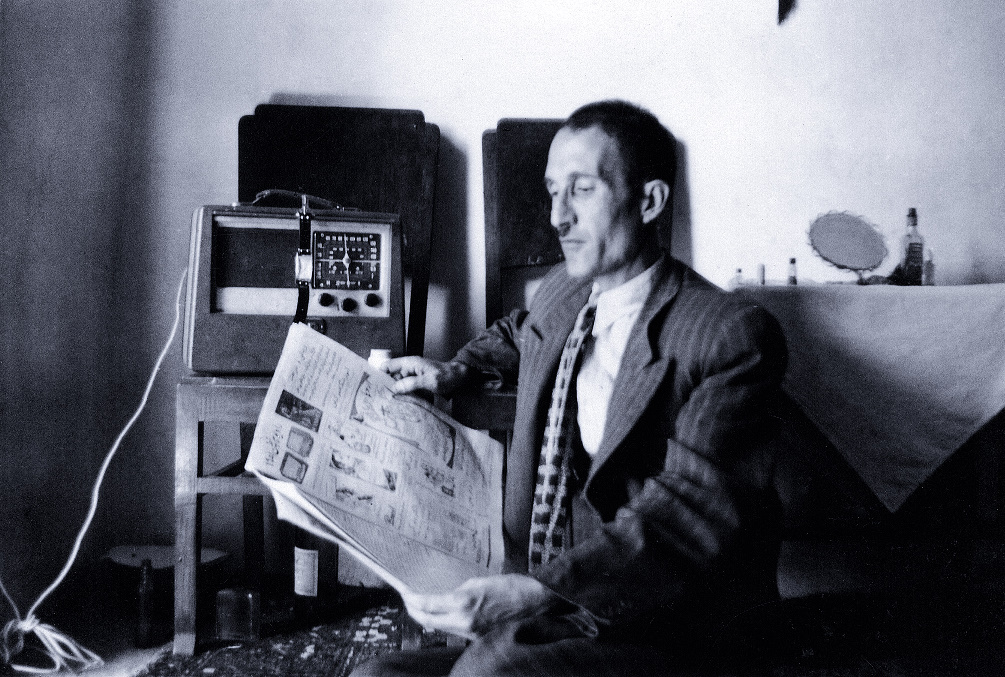
\includegraphics[width=0.55\textwidth]{mahmood-with-newspaper-259125453-bg.jpg}}
\caption{My wife's father reading a newspaper 1955.}
\label{fig:4048X0}
\end{figure}

Such crimes against imagery are common. My maternal grandmother was also
a keen \emph{unorganized} photographer. She~didn't~label prints or
neatly file slides but she shot everything that caught her eye. Over six
decades she piled up thousands of images, but when she moved into town,
she accidentally sold stacks of what she thought were empty slide
carousels to yard sale strangers. Some of the carousels were empty but
the rest held the bulk or her slide collection. The surviving images,
like this \hyperlink{ht:4048X1}{old Kodachrome of my great-grandmother and her sister},
constantly remind me of all the great shots I will never see! Don't
trash your family pictures you will grow to regret it.

%{[}caption id=``attachment\_4060'' align=``aligncenter''  width=``332''{]}
%\href{http://conceptcontrol.smugmug.com/People/From-Hazels-Albums-1/7104752\_FZK4j4\#!i=475252263\&k=s7FVxLV\&lb=1\&s=A}{\includegraphics{great-grandma-raver-with-sister-maude-1950s.jpg}}
%My great-grandmother (light blue dress) and her sister
%1950s.
%{[}/caption{]}

\begin{figure}[htbp]
\centering
\hypertarget{ht:4048X1}{}
\href{http://conceptcontrol.smugmug.com/People/From-Hazels-Albums-1/7104752\_FZK4j4\#!i=475252263\&k=s7FVxLV\&lb=1\&s=A}{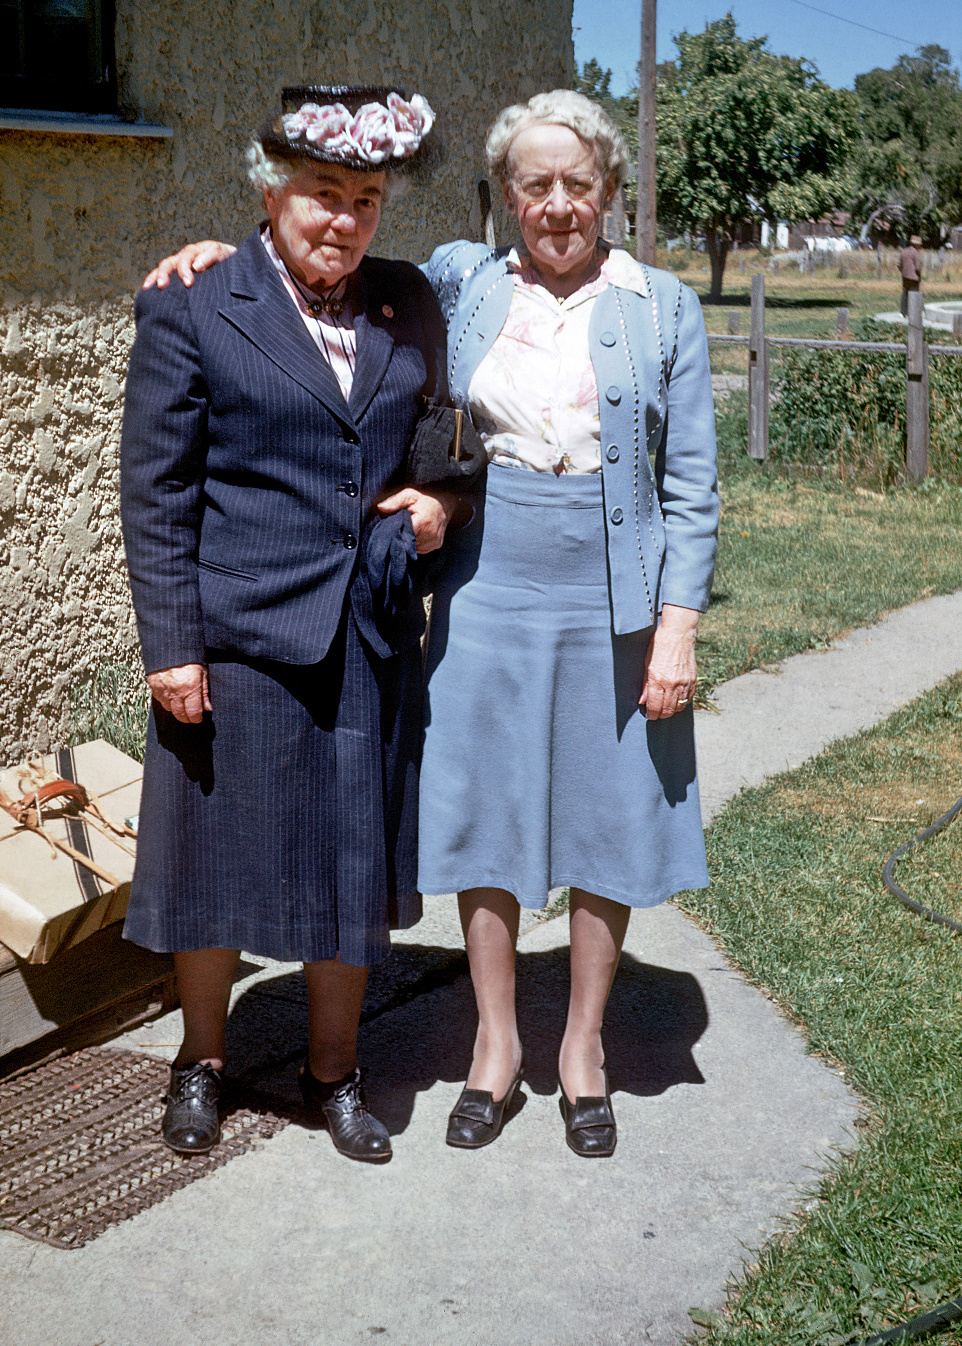
\includegraphics[width=0.40\textwidth]{great-grandma-raver-with-sister-maude-1950s-bg.jpg}}
\caption{My great-grandmother (light blue dress) and her sister 1950s.}
\label{fig:4048X1}
\end{figure}

My mother's recently recovered stash held a few gems I had never seen
like this \hyperlink{ht:4048X2}{great little snapshot of my maternal grandmother with her two
daughters}: my late mother as a pouty girl and my aunt as a baby. The old
car in the background would be marked down as a ``distracting element''
in many photography classes. This merely shows how bad the advice and
guidelines dispensed in such courses can be. The car is an essential
element; it turns a nice snapshot into a sweet period piece.

%{[}caption id=``attachment\_4067'' align=``aligncenter''  width=``360''{]}
%\href{http://conceptcontrol.smugmug.com/People/From-Hazels-Albums-1/7104752\_FZK4j4\#!i=2524884643\&k=WcQmrR4\&lb=1\&s=A}{\includegraphics{hazel-evelyn-alberta-car-1940.jpg}}
%Hazel, Alberta (baby) and Evelyn 1940.
%{[}/caption{]}

\begin{figure}[htbp]
\centering
\hypertarget{ht:4048X2}{}
\href{http://conceptcontrol.smugmug.com/People/From-Hazels-Albums-1/7104752\_FZK4j4\#!i=2524884643\&k=WcQmrR4\&lb=1\&s=A}{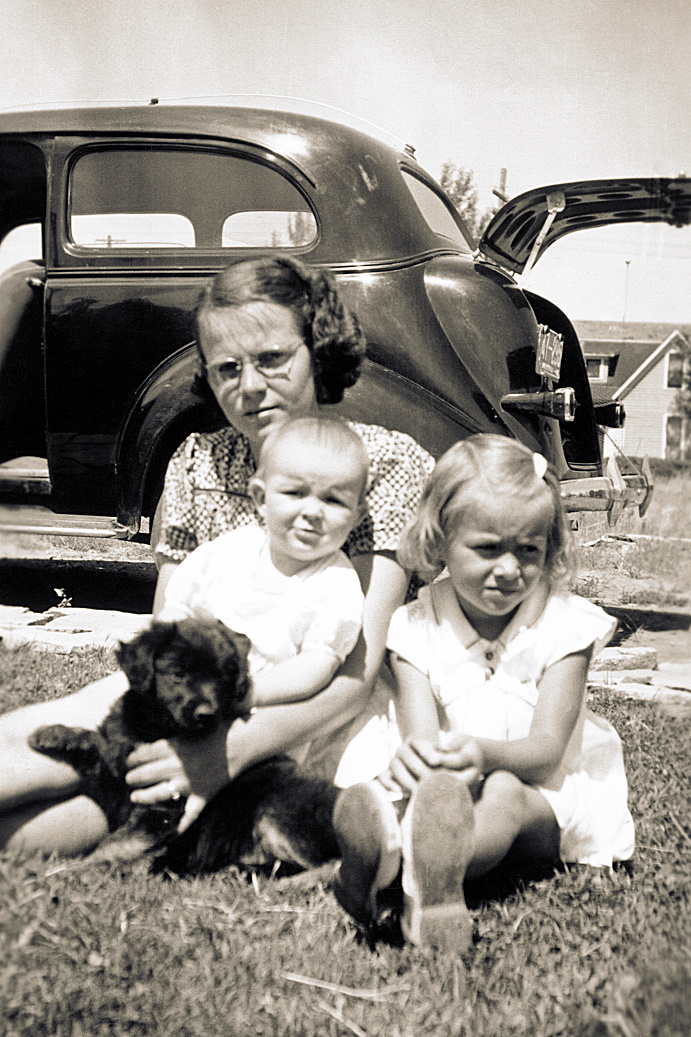
\includegraphics[width=0.40\textwidth]{hazel-evelyn-alberta-car-1940-bg.jpg}}
\caption{Hazel, Alberta (baby) and Evelyn 1940.}
\label{fig:4048X2}
\end{figure}

Here's another \hyperlink{ht:4048X3}{snapshot of my mother and aunt with a puppy}. This picture
is almost seventy years old but I still see the same expression on my
aunt's face. Your smile is a lifelong affliction; I would recommend
getting used to it.

%{[}caption id=``attachment\_4069'' align=``aligncenter''  width=``400''{]}
%\href{http://conceptcontrol.smugmug.com/People/From-Hazels-Albums-1/7104752\_FZK4j4\#!i=2525057933\&k=DsggvtX\&lb=1\&s=A}{\includegraphics{evelyn-alberta-puppy-1944.jpg}}
%Evelyn and Alberta with puppy 1944.
%{[}/caption{]}

\begin{figure}[htbp]
\centering
\hypertarget{ht:4048X3}{}
\href{http://conceptcontrol.smugmug.com/People/From-Hazels-Albums-1/7104752\_FZK4j4\#!i=2525057933\&k=DsggvtX\&lb=1\&s=A}{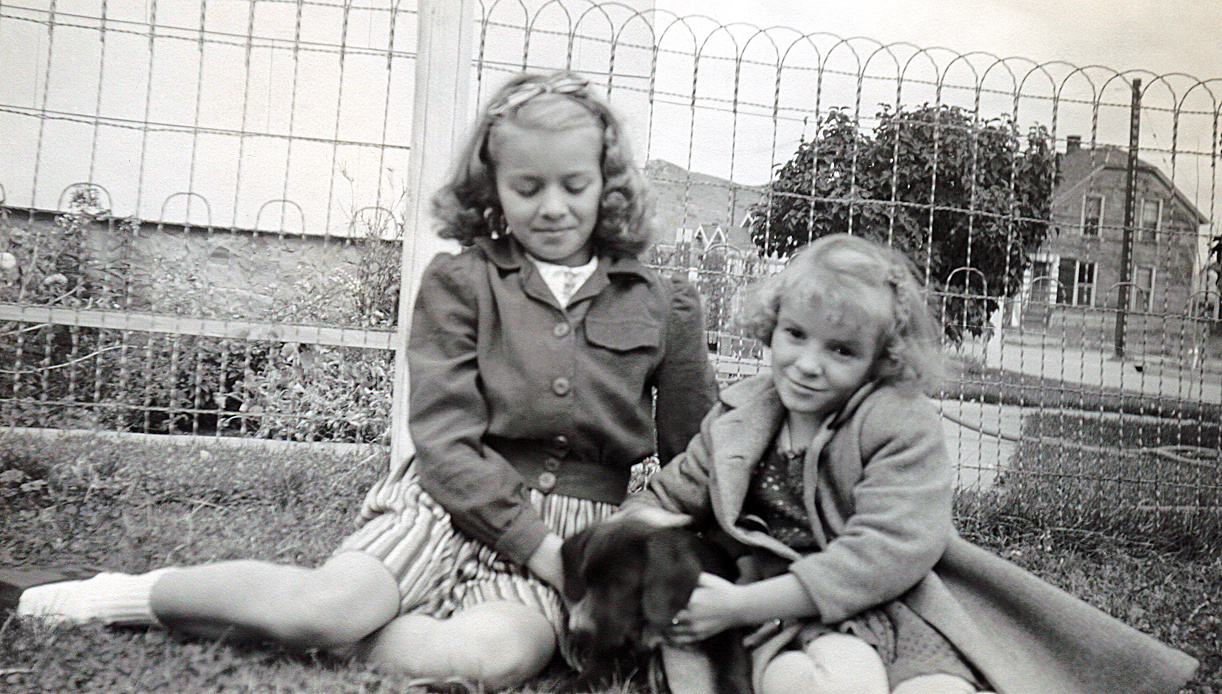
\includegraphics[width=0.50\textwidth]{evelyn-alberta-puppy-1944-bg.jpg}}
\caption{Evelyn and Alberta with puppy 1944.}
\label{fig:4048X3}
\end{figure}

Along with the \emph{amateur} snapshots a number of professional studio
portraits turned up. The following is a \hyperlink{ht:4048X4}{hand tinted print of my mother}
as a ten-year old. Color photography obliterated the art of hand
tinting. It is rarely seen outside of photographic art classes today.
Tinting is often unnatural and hokey but it sometimes lends an eerie
painting quality. Here the tinting works. Tinted prints are becoming
rare and valuable. Don't throw them away!

%{[}caption id=``attachment\_4057'' align=``aligncenter''  width=``302''{]}
%\href{http://conceptcontrol.smugmug.com/People/From-Hazels-Albums-1/7104752\_FZK4j4\#!i=2521568789\&k=sg9BR5f\&lb=1\&s=A}{\includegraphics{evelyn-eggar-studio-tinted-1945.jpg}}
%Evelyn age ten hand tinted 1945.
%{[}/caption{]}

\begin{figure}[htbp]
\centering
\hypertarget{ht:4048X4}{}
\href{http://conceptcontrol.smugmug.com/People/From-Hazels-Albums-1/7104752\_FZK4j4\#!i=2521568789\&k=sg9BR5f\&lb=1\&s=A}{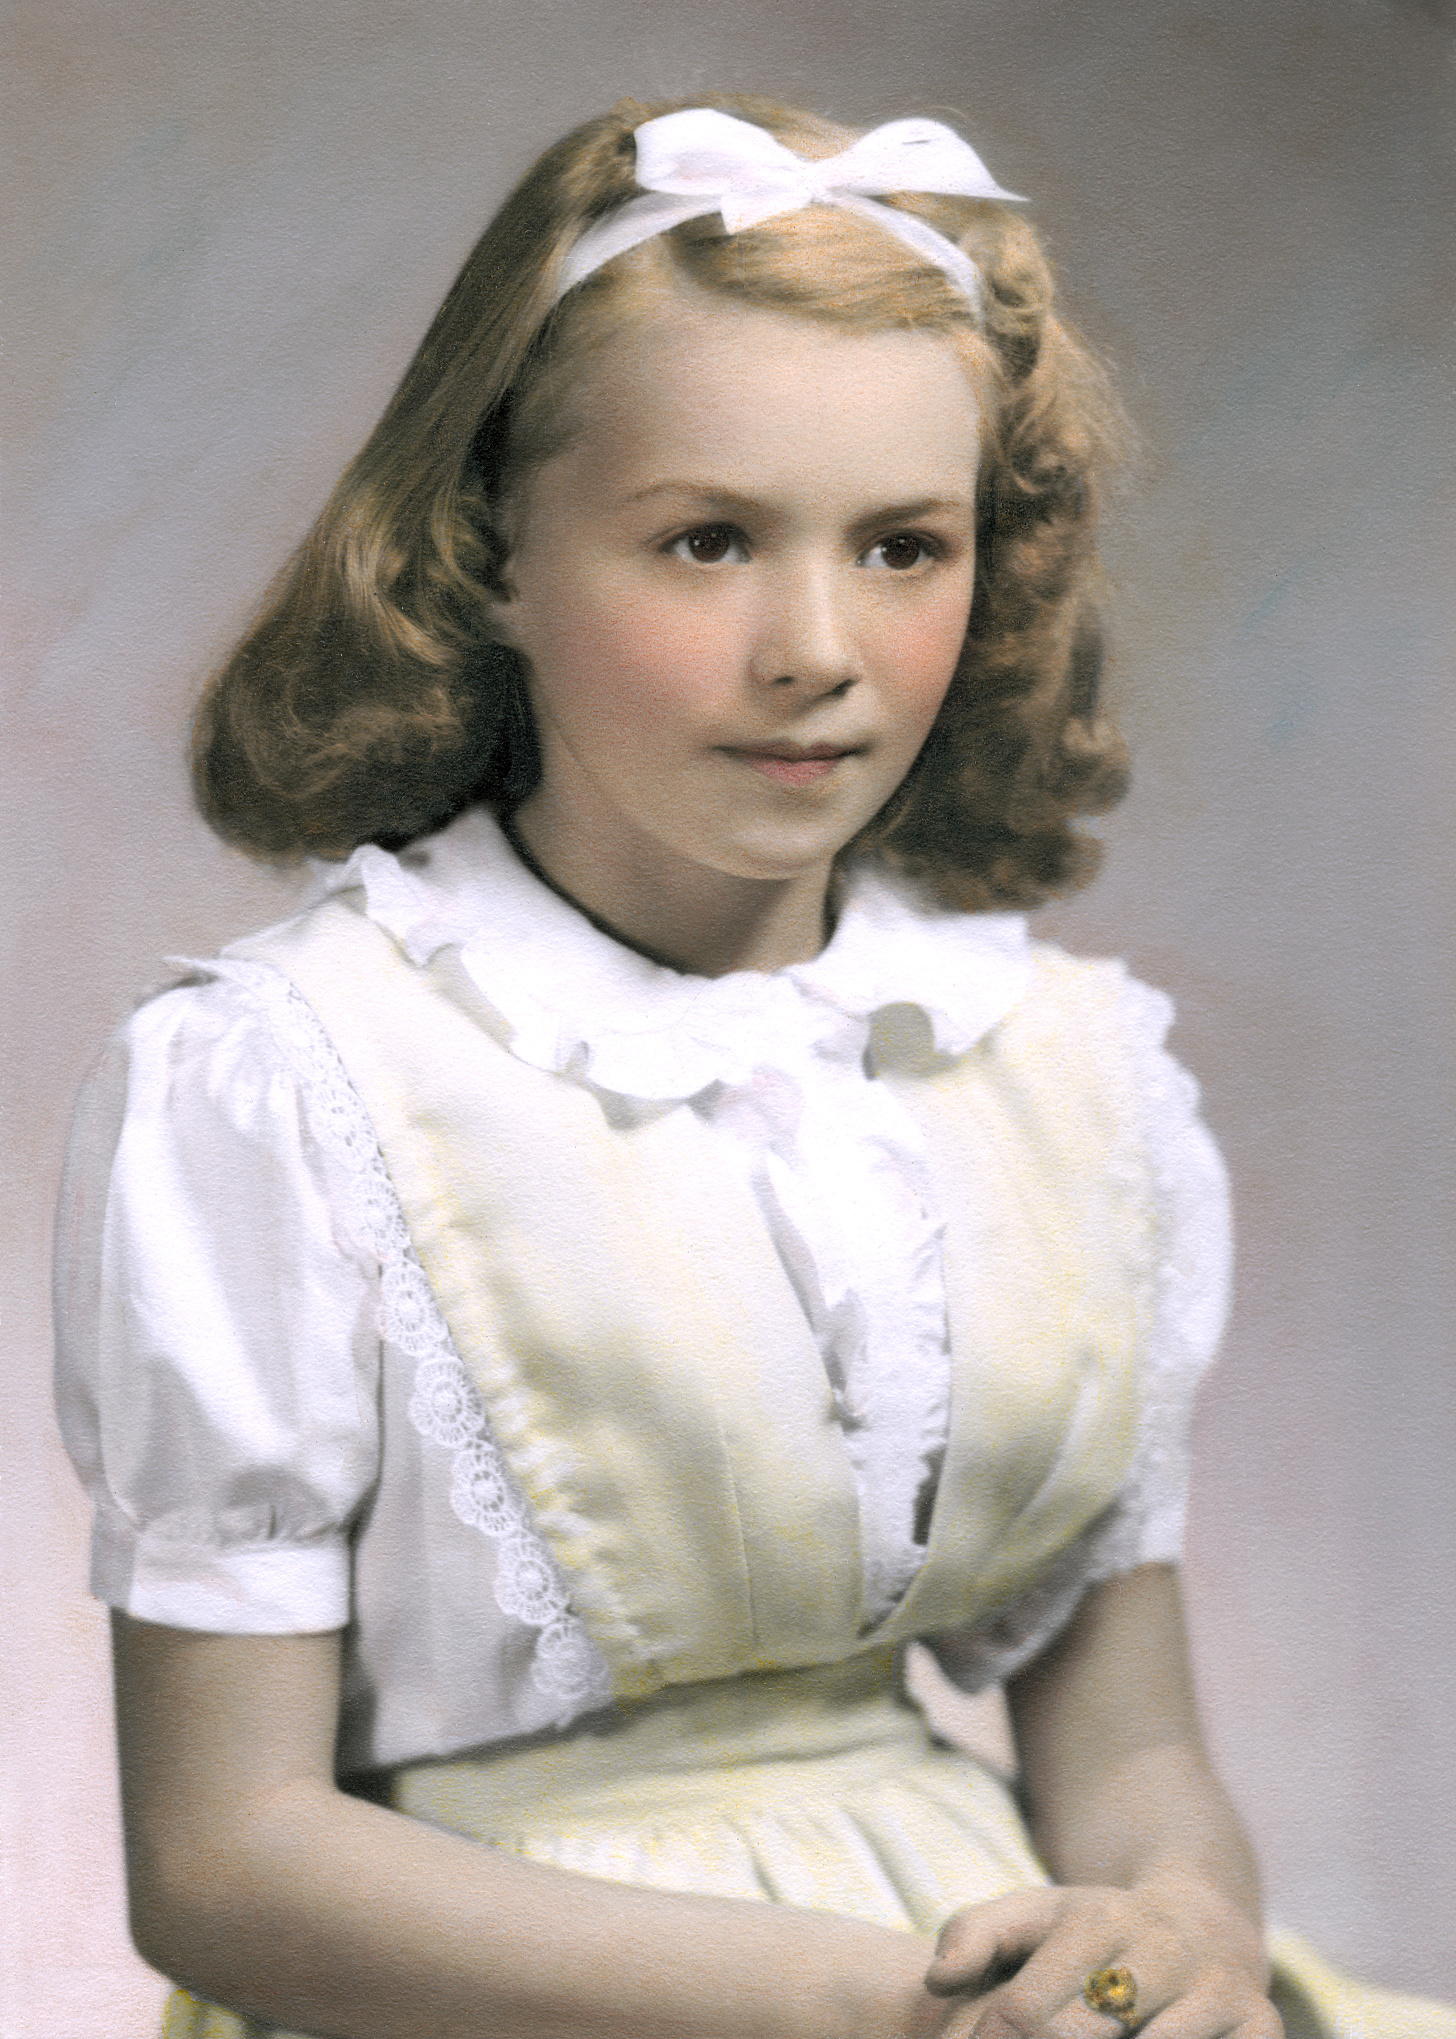
\includegraphics[width=0.60\textwidth]{evelyn-eggar-studio-tinted-1945-bg.jpg}}
\caption{Evelyn age ten hand tinted 1945.}
\label{fig:4048X4}
\end{figure}

\newpage %inner-\newpage - will require tweaks if page size changes

Finally, here's a wonderful never seen \hyperlink{ht:4048X5}{portrait of my mother as an
eleven year old}. This may be the best portrait of my mother at any age.
The studio photographer caught her in the middle of a great smile. This
picture was taken over six decades ago but I doubt that modern imaging
technology could significantly improve it.

%{[}caption id=``attachment\_4056'' align=``aligncenter''  width=``320''{]}
%\href{http://conceptcontrol.smugmug.com/People/From-Hazels-Albums-1/7104752\_FZK4j4\#!i=2521568625\&k=86Sn8rs\&lb=1\&s=A}{\includegraphics{evelyn-eggar-bruno-studio-portrait.jpg}}
%Evelyn age eleven studio portrait 1946.
%{[}/caption{]}

\begin{figure}[htbp]
\centering
\hypertarget{ht:4048X5}{}
\href{http://conceptcontrol.smugmug.com/People/From-Hazels-Albums-1/7104752\_FZK4j4\#!i=2521568625\&k=86Sn8rs\&lb=1\&s=A}{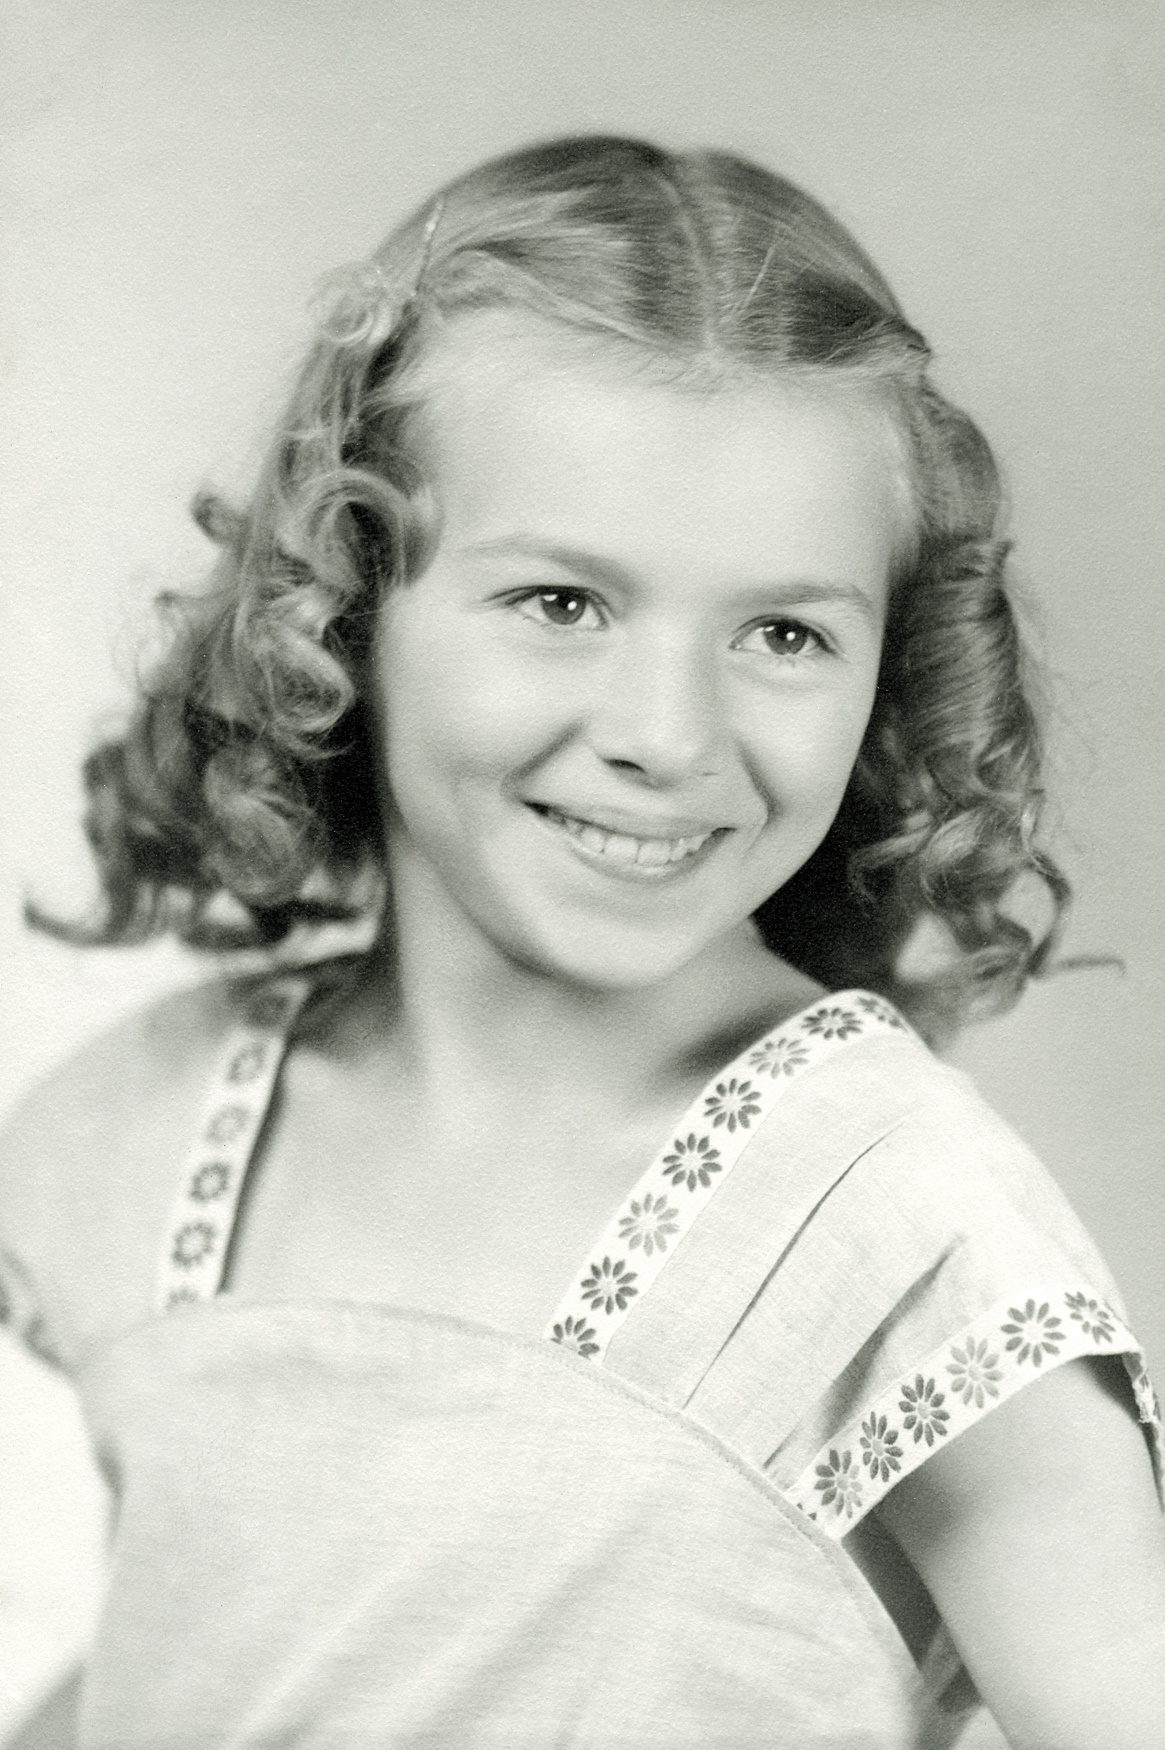
\includegraphics[width=0.60\textwidth]{evelyn-eggar-bruno-studio-portrait-bg.jpg}}
\caption{Evelyn age eleven studio portrait 1946.}
\label{fig:4048X5}
\end{figure}

Finding this portrait shortly after my mother's death took away some of
the sting. I had a great mother, and because I treat family pictures
with the respect they deserve, I have the photographic evidence to prove
it.

%\captionsetup[floatingfigure]{labelformat=empty}
%\begin{figure}[htbp]
%\begin{floatingfigure}[l]{0.25\textwidth}
%\centering
%\includegraphics[width=0.23\textwidth]{mahmood-with-newspaper-259125453.jpg}
%\caption{~~~IMCAPTION~~~}
%\label{fig:4048X0}
%\end{floatingfigure}
%\end{figure}

%\captionsetup[floatingfigure]{labelformat=empty}
%\begin{figure}[htbp]
%\begin{floatingfigure}[l]{0.25\textwidth}
%\centering
%\includegraphics[width=0.23\textwidth]{great-grandma-raver-with-sister-maude-1950s.jpg}
%\caption{~~~IMCAPTION~~~}
%\label{fig:4048X1}
%\end{floatingfigure}
%\end{figure}

%\captionsetup[floatingfigure]{labelformat=empty}
%\begin{figure}[htbp]
%\begin{floatingfigure}[l]{0.25\textwidth}
%\centering
%\includegraphics[width=0.23\textwidth]{hazel-evelyn-alberta-car-1940.jpg}
%\caption{~~~IMCAPTION~~~}
%\label{fig:4048X2}
%\end{floatingfigure}
%\end{figure}

%\captionsetup[floatingfigure]{labelformat=empty}
%\begin{figure}[htbp]
%\begin{floatingfigure}[l]{0.25\textwidth}
%\centering
%\includegraphics[width=0.23\textwidth]{evelyn-alberta-puppy-1944.jpg}
%\caption{~~~IMCAPTION~~~}
%\label{fig:4048X3}
%\end{floatingfigure}
%\end{figure}

%\captionsetup[floatingfigure]{labelformat=empty}
%\begin{figure}[htbp]
%\begin{floatingfigure}[l]{0.25\textwidth}
%\centering
%\includegraphics[width=0.23\textwidth]{evelyn-eggar-studio-tinted-1945.jpg}
%\caption{~~~IMCAPTION~~~}
%\label{fig:4048X4}
%\end{floatingfigure}
%\end{figure}

%\captionsetup[floatingfigure]{labelformat=empty}
%\begin{figure}[htbp]
%\begin{floatingfigure}[l]{0.25\textwidth}
%\centering
%\includegraphics[width=0.23\textwidth]{evelyn-eggar-bruno-studio-portrait.jpg}
%\caption{~~~IMCAPTION~~~}
%\label{fig:4048X5}
%\end{floatingfigure}
%\end{figure}



%\end{document}